\vspace{-1mm}
\section{Sorunun A\c{c}{\i}klamas{\i}}
%
% \begin{wrapfigure}{r}{0.4\textwidth} %this figure will be at the right
%     \vspace{-5mm}
%     \centering
%     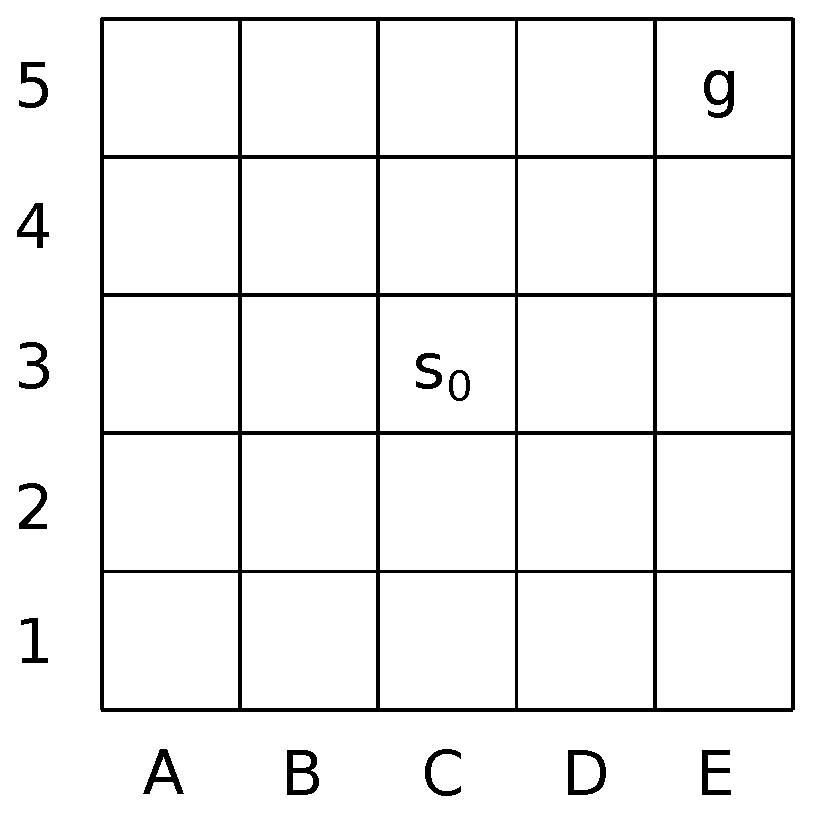
\includegraphics[width=0.25\textwidth]{./figures/drawing.eps}
%     \caption{Problemin \c{s}emati\u{g}i}
%     \label{fig:schematic}
%     \vspace{-5mm}
% \end{wrapfigure}
%
Dinwen kasabasinin 15 yasindaki dahi cocugu Sonaj, kendisini bulundugu andan 33
yil ileriye veya geriye aninda goturebilen bir zaman makinesi icat etmistir,
fakat bu makinenin iki zaafi vardir: 1) bu makine her yolculuk icin, yarilanma
omru tam 11 yil olan ve cok ender bulunabilen Secium 731 maddesinin 1 mg'ini
kullanmaktadir ve 2) her yolculugun arasinda en az 11 yil beklemek
gerekmektedir.

Elinde 21 mg Secium 731 bulunan Sonaj zamanda yolculuga cikmis, zamanda
gorebilecegi en ileri tarihi gormus ve basladigi gune geri donebilmistir. Sonaj
yolculuk suresince yeni Secium 731 bulmamistir. Zaman yolculuklari aninda
gerceklestiginden, bu yolculuklar sirasinda Sonaj hic yaslanmamaktadir ve Secium
731 miktari, yolculuk icin gereken 1 mg disinda azalmamaktadir.

Sonaj'in geri dondugundeki yasina $\alpha$, elinde kalan Secium 731'in mg
cinsinden miktarina $\beta$, Sonaj'in zaman yolculugna basladigi gun ile bugune 
en uzak oldugu an arasindaki yil cinsinden farka da $\gamma$ diyelim.

Buna gore $\alpha + \beta + \gamma$ kactir?